%%This is a standard LaTeX2e article document template. personal version 12/5/200%%
\documentclass[11pt,twoside]{article}
%%%%%%%%%%%%%%%%%%%%%%%%%%%%%%%packages%%%%%%%%%%%%%%%%%%%%%%%%%%%%%%%%%%%%%%%%%%%%%%%%%%%%%%%%%%
\pagestyle{empty}

\usepackage{latexsym}
\usepackage{amssymb}
\usepackage{amsfonts}
\usepackage{amstext}
\usepackage{amsmath}
\usepackage{amsthm}
\usepackage{multicol}
\usepackage{hyperref}
\usepackage{graphicx}
\usepackage{tikz}
\usepackage{wrapfig}
\usepackage{enumitem}

%%%%%%%%%%%%%%%%%%%%%%%%%%%%%%%formatting%%%%%%%%%%%%%%%%%%%%%%%%%%%%%%%%%%%%%%%%%%%%%%%%%%%%%%%
\setlength{\topmargin}{-.1in}        %%%  This sets all the spacing stuff to use the page more
\setlength{\oddsidemargin}{0in}    %%%  efficiently than the normal "article" setup would.
\setlength{\evensidemargin}{0in}   %%%  It's OK to play with these some.
\setlength{\textheight}{9in}     %%%
\setlength{\textwidth}{6.25in}     %%%
\setlength{\headsep}{0in}          %%%
\setlength{\headheight}{0in}       %%%
%\setlength{\footskip}{0in}         %%%

%%%%%%%%%%%%%%%%%%%%%%%%%%%%%%%%%%%%%%%%%%%%%%%%%%%%%%%%%%%%%%%%%%%%%%%%%%%%%%%%%%%%%%%%%%%%%%%

\begin{document}

\begin{center}
{\bf \Large Math 335, Homework 3}\\
\vspace{0.1in}
{\Large Due Wednesday, February 17}
\vspace{0.1cm}
\end{center}

\hrule

\vspace{.2in}

\begin{enumerate}

\item Let $A$, $B$, and $C$ be sets, and let $f: A \rightarrow B$ and $g: B \rightarrow C$ be functions.

\begin{enumerate}[label=(\alph*)]
\item Prove that if $f$ and $g$ are injective, then $g \circ f$ is injective.

\begin{proof}[\color{red}Proof.]
Assume $f\colon A\to B$ and $g\colon B \to C$ are injective functions.  Then by definition, $\forall a_1, a_2 \in A$,
\[ f(a_1) = f(a_2) \implies a_1 = a_2, \]
and $\forall b_1, b_2 \in B$,
\[ g(b_1) = g(b_2) \implies b_1 = b_2. \]
To prove $g \circ f$ is injective, we must show that
\[ (g\circ f)(a_1) = (g\circ f)(a_2) \implies a_1 = a_2. \]
Assume $g(f(a_1)) = g(f(a_2))$.  Notice that by applying $f(a_1) = b_1$ and $f(a_2) = b_2$ to our injective function $g$, we can conclude that $b_1 = b_2 = f(a_1) = f(a_2)$.  Since $f$ is also injective, $a_1 = a_2$.  Hence $g\circ f$ is injective.
\end{proof}

\item Prove that if $f$ and $g$ are surjective, then $g \circ f$ is surjective.

\begin{proof}[\color{red}Proof.]
Assume $f\colon A\to B$ and $g\colon B \to C$ are surjective functions.  Then by definition, this means $\forall b\in B$ there exists $a\in A$ such that $f(a) = b$.  Similarly, for every $c\in C$, there exists $f(a)=b\in B$ such that $g(b) = g(f(a)) = c$.  Hence $g\circ f$ is surjective.
\end{proof}

\end{enumerate}

\vspace{0.5cm}

\item Prove that a function $f: A \rightarrow B$ is both injective and surjective if and only if it has an inverse function $f^{-1}: B \rightarrow A$.

\begin{proof}[\color{red}Proof.]
For the forward direction, assume $f\colon A\to B$ is bijective.  Since $f$ is surjective, $\forall b\in B$, $\exists a\in A$ such that $f(a) = b$.  Let $b\in B$ and define a function $f^{-1}\colon B \to A$ such that $f^{-1}(b) = a$.  Since $f$ is injective, $f(a_1) = f(a_2) \implies a_1 = a_2$, so each $a\in A$ is unique as is each $b\in B$.

Notice that $(f\circ f^{-1})(b) = f(f^{-1}(b)) = f(a) = b$ and $(f^{-1}\circ f)(a) = f^{-1}(f(a)) = f^{-1}(b) = a$, which means that $f^{-1}$ is the inverse of $f$.

Conversely, assume that $f\colon A\to B$ has an inverse $f^{-1}\colon B\to A$.  To prove that $f$ is surjective, we must show that $\forall b\in B$ there exists $a\in A$ such that $f(a) = b$.  Let $b\in B$ and $f^{-1}(b) = a$.  Then $f(a) = f(f^{-1}(b)) = b$.

To prove that $f$ is injective, assume $a_1, a_2 \in A$ and $f(a_1) = f(a_2) = b$.  We must show that $a_1 = a_2$.  Suppose that $f^{-1}(b) = a$.  Notice that
\begin{align*}
a_1 &= (f^{-1}\circ  f)(a_1) = f^{-1}(f(a_1))\\
&= f^{-1}(b) = a.
\end{align*}
Also,
\begin{align*}
a_2 &= (f^{-1}\circ  f)(a_2) = f^{-1}(f(a_2))\\
&= f^{-1}(b) = a.
\end{align*}
Hence $a_1=a=a_2$, which means that $f$ is injective.
\end{proof}

\vspace{0.5cm}

\item Consider the following two elements of $S_8$, written in cycle notation:
\[f = (2,3,8,4,7) \; (5,6) \]
\[ g= (1,2,3,4,5) \; (6,7,8).\]

\begin{enumerate}[label=(\alph*)]
\item Write $f$ in function notation.  (That is, write $f(1) = \cdots, f(2) = \cdots$, et cetera.)

{\color{red}Answer:}

\begin{tabular}{ r r r r }
$f(1) = 1$	& $f(3) = 8$	& $f(5) = 6$	& $f(7) = 2$\\
$f(2) = 3$	& $f(4) = 7$	& $f(6) = 5$	& $f(8) = 4$
\end{tabular}

\item Compute $f^{-1}$.  Express your answer in cycle notation.

{\color{red}Answer:}

$f^{-1} = (2,7,4,8,3)(5,6)$

\begin{tabular}{ r r r r }
$f^{-1}(1) = 1$	&	$f^{-1}(3) = 2$	&	$f^{-1}(5) = 6$	&	$f^{-1}(7) = 4$\\
$f^{-1}(2) = 7$	&	$f^{-1}(4) = 8$	&	$f^{-1}(6) = 5$	&	$f^{-1}(8) = 3$
\end{tabular}

\item Compute $f \circ g$.  Express your answer in cycle notation, with each number only appearing once.

{\color{red}Answer:}

$f\circ g = (1,3,7,4,6,2,8,5)$
\end{enumerate}

\vspace{0.5cm}

\item A {\it transposition} is defined as an element of $S_n$ that swaps two numbers but sends every other number to itself; for example, $(2,5)$ is a transposition in $S_5$ that swaps $2$ and $5$.
\begin{enumerate}[label=(\alph*)]
\item Express the element
\[f = (2,4,5)\]
of $S_5$ as a composition of two transpositions.

{\color{red}Answer:}

$f\circ g$

$g = (2,5)$\\
$f = (4,5)$

\item Express the element
\[g = (1,2,3,4)\]
of $S_4$ as a composition of transpositions.  ({\bf Hint}: If you want to send $2$ to $3$, you can first swap $1$ and $2$ and then swap $1$ and $3$.)

{\color{red}Answer:}

$f\circ g$

$g = (1,3)$\\
$f = (1,4)(2,3)$

Also

$g = (1,2)(3,4)$\\
$f = (1,3)$

\end{enumerate}
In fact, it's a theorem that every element of $S_n$ can be expressed as a composition of transpositions.  We won't cover this theorem in class, but you can find a proof in Gallian.

\vspace{0.5cm}

\item Explain in words how the group $D_4$ of symmetries of a square can be viewed as a subset of the symmetric group $S_4$.  Are all elements of $S_4$ symmetries of a square?

{\color{red}Answer:}

Let us consider the symmetries of a square from the diagram below:

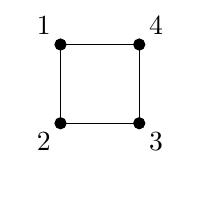
\begin{tikzpicture}
	\draw (0,1) -- (1,1) -- (1,0) -- (0,0) -- (0,1);
	\filldraw[black] (0,1) circle (2pt) node[anchor=south east] {1};
	\filldraw[black] (0,0) circle (2pt) node[anchor=north east] {2};
	\filldraw[black] (1,0) circle (2pt) node[anchor=north west] {3};
	\filldraw[black] (1,1) circle (2pt) node[anchor=south west] {4};
\end{tikzpicture}

The group $D_4$ can be then described as follows:\\
Counterclockwise rotation: $r = (1,2,3,4)$\\
Horizontal reflection: $h = (1,2)(3,4)$\\
Vertical reflection: $v = (1,4)(2,3)$\\
Diagonal reflection (along the 1 \& 3 axis): $d = (2,4)$\\
Diagonal reflection (along the 2 \& 4 axis): $d' = (1,3)$

Each of these operations on the symmetries of a square are a member of the symmetric group $S_4$.  In addition, all symmetries of the square can be produced by a composition of these operations.  Nevertheless, not all elements of $S_4$ are symmetries of a square.  As a counterexample, $f = (1,2)$ is not a member of the group $D_4$ as it will not produce a valid square.
\end{enumerate}


%\newpage
%
%\begin{center}
%{\bf \Large Extra Credit Opportunity: Mathematical Writing}\\
%\vspace{0.1in}
%{\Large Turn in anytime before Wednesday, February 24}
%\vspace{0.1cm}
%\end{center}
%
%\hrule
%
%\vspace{.2in}
%
%You'll be doing a lot of writing in this course, in the form of mathematical proofs and (at the end of the semester) a final project.  Writing about mathematics is a hard skill that takes a lot of practice, and it also has many peculiar conventions that make it different from writing more generally.
%
%For this extra credit opportunity, your assignment is the following:
%\begin{enumerate}
%\item Read the two articles \href{http://danaernst.com/teaching/ElementsOfStyle.pdf}{``Elements of Style for Proofs"} by D. C. Ernst and \href{https://math.hmc.edu/su/wp-content/uploads/sites/10/2019/11/good-math-writing.pdf}{``Guidelines for Good Mathematical Writing"} by Francis Su.  (The titles in the previous sentence are clickable links to the articles.)
%\item Write a paragraph summarizing your thoughts on the tips in these articles.  For example, you might comment on whether you found any of them surprising or motivating.
%\item Identify at least two specific things you learned from these articles that you want to work on this semester in your own mathematical writing.
%\end{enumerate}
%Your responses can be hand-written or typed.  They should be sent by Wednesday, February 24th (the day of our first exam) to me via e-mail, at eclader@sfsu.edu.
%
%\vspace{0.5cm}
%
%A thoughtful response to this assignment will earn you {\bf 5 points} extra credit.

\end{document}
